%%%%%%%%%%%%%%%%%%%%%%%%%%%%%%%%%%%%%%%%%%%%%%%%%%%%%%%%%%%%%
%% Begin exercise %%
%%%%%%%%%%%%%%%%%%%%%%%%%%%%%%%%%%%%%%%%%%%%%%%%%%%%%%%%%%%%%
\ex{Zero-voltage switching in PWM converters}

%%%%%%%%%%%%%%%%%%%%%%%%%%%%%%%%%%%%%%%%%%%%%%%%%%%%%%%%%%%%%
%% Task 1 %%
%%%%%%%%%%%%%%%%%%%%%%%%%%%%%%%%%%%%%%%%%%%%%%%%%%%%%%%%%%%%%

\task{Charge and energy of the ZVS transition}

A half-bridge operates at $V_\mathrm{DC}=\SI{48}{\volt}$ (Fig.~\ref{fig:ex08_hb}). The output capacitance of each \SI{100}{\volt} GaN transistor is approximated by
\begin{equation}
	C_\mathrm{oss}(v)=\frac{C_0}{\sqrt{1+v/V_\mathrm{j}}},\qquad C_0=\SI{443}{\pico\farad},\quad V_\mathrm{j}=\SI{5}{\volt}.
\end{equation}
During the dead time both transistors are off. The inductor $L$ connects the switch node to a constant voltage $V_x$; at the start of the dead time it carries the current $I_0$ into the switch node, which rises from 0 to $V_\mathrm{DC}$.

%%%%%%%%%%%%%%%%%%%%%%%%%%%%%%%%%%%%%%%%%%%%%%%%%%%%%%%%%%%%%%%%%%%%%%%%%%
% Half-bridge during the dead time (Exercise 08, Tasks 1 and 2)
%%%%%%%%%%%%%%%%%%%%%%%%%%%%%%%%%%%%%%%%%%%%%%%%%%%%%%%%%%%%%%%%%%%%%%%%%%

\begin{figure}[htb]
	\begin{center}
		\begin{circuitikz}[scale=0.9, transform shape]
			\draw (0,0) to[V, l=$V_\mathrm{DC}$] (0,4) -- (2,4);
			\draw (2,4) to[C, l_=$C_\mathrm{oss}$] (2,2) to[C, l_=$C_\mathrm{oss}$] (2,0);
			\draw (2,4) -- (3.4,4) node[nigfete, anchor=D] (HS) {};
			\draw (0,0) -- (3.4,0) node[nigfete, anchor=S] (LS) {};
			\draw (HS.S) -- (LS.D);
			\draw (2,2) -- (3.4,2) node[circ]{};
			\draw (3.4,2) to[short, i=$i_L$] (4.8,2) to[L, l=$L$] (6.6,2);
			\draw (3.4,0) -- (6.6,0) to[V, l_=$V_x$] (6.6,2);
			\draw (1,0) node[ground]{};
			\node[anchor=south east, inner sep=1pt] at (3.35,2.05) {$v_\mathrm{sw}$};
			\node[anchor=west] at (3.9,3.45) {high side};
			\node[anchor=west] at (3.9,0.55) {low side};
		\end{circuitikz}
	\end{center}
	\caption{Half-bridge during the dead time: both transistors are off, the inductor current charges the switch node. Each $C_\mathrm{oss}$ depends on the drain-source voltage of its own transistor.}
	\label{fig:ex08_hb}
\end{figure}


\subtask{Calculate $Q_\mathrm{oss}$ and $E_\mathrm{oss}$ at \SI{48}{\volt} and the charge- and energy-equivalent capacitances $C_\mathrm{o(tr)}$ and $C_\mathrm{o(er)}$. Hint: substitute $u=1+v/V_\mathrm{j}$.}

\begin{solutionblock}
	\begin{equation}
		Q_\mathrm{oss}(V)=\int_0^VC_\mathrm{oss}\,\mathrm{d}v=2C_0V_\mathrm{j}\left(\sqrt{1+V/V_\mathrm{j}}-1\right)=2\cdot\SI{443}{\pico\farad}\cdot\SI{5}{\volt}\cdot(3.256-1)=\SI{10.0}{\nano\coulomb}
	\end{equation}
	\begin{equation}
		E_\mathrm{oss}(V)=\int_0^Vv\,C_\mathrm{oss}\,\mathrm{d}v=C_0V_\mathrm{j}^2\left[\frac{2}{3}\left(u^{3/2}-1\right)-2\left(u^{1/2}-1\right)\right]_{u=10.6}=\SI{443}{\pico\farad}\cdot\SI{25}{\volt\squared}\cdot17.83=\SI{0.197}{\micro\joule}
	\end{equation}
	$C_\mathrm{o(tr)}=Q_\mathrm{oss}/V=\SI{208}{\pico\farad}$, $C_\mathrm{o(er)}=2E_\mathrm{oss}/V^2=\SI{171}{\pico\farad}$. The small-signal value at \SI{48}{\volt} is only $\SI{136}{\pico\farad}$.
\end{solutionblock}

\subtask{A stiff current of \SI{5}{\ampere} charges the node. Calculate the transition time and compare it with estimates based on $C_\mathrm{o(er)}$ and on the small-signal $C_\mathrm{oss}(\SI{48}{\volt})$.}

\begin{solutionblock}
	The current moves the charge of both capacitances: $t_\mathrm{tr}=2Q_\mathrm{oss}/I=\SI{4.0}{\nano\second}$. With $C_\mathrm{o(er)}$: $2\cdot\SI{171}{\pico\farad}\cdot\SI{48}{\volt}/\SI{5}{\ampere}=\SI{3.3}{\nano\second}$ (18\,\% too short); with $C_\mathrm{oss}(\SI{48}{\volt})$: $\SI{2.6}{\nano\second}$ (35\,\% too short). A dead time based on them would cut the transition short. Time and charge go with $C_\mathrm{o(tr)}$.
\end{solutionblock}

\subtask{Calculate the energy that the inductor delivers during the transition for $V_x=0$, 12 and \SI{24}{\volt} and compare it with $2E_\mathrm{oss}$. Where does this energy go?}

\begin{solutionblock}
	$W=Q_\mathrm{oss}(V_\mathrm{DC}-2V_x)$: $\SI{0.48}{\micro\joule}$, $\SI{0.24}{\micro\joule}$ and 0. For $V_x=0$ the estimate $2E_\mathrm{oss}=\SI{0.395}{\micro\joule}$ is 18\,\% too low.
	The stored energies only swap: the low-side capacitance gains $E_\mathrm{oss}$, the high-side capacitance loses $E_\mathrm{oss}$. Its charge $Q_\mathrm{oss}$ is pushed back into the bus at \SI{48}{\volt}, which takes up $Q_\mathrm{oss}V_\mathrm{DC}=\SI{0.48}{\micro\joule}$. The source $V_x$ supplies $2Q_\mathrm{oss}V_x$, the inductor the rest. Nothing is dissipated.
\end{solutionblock}

\subtask{The inductor has $L=\SI{225}{\nano\henry}$. Which initial current is needed for complete ZVS with $V_x=0$ and with $V_x=\SI{12}{\volt}$? What limits ZVS for $V_x=\SI{24}{\volt}$?}

\begin{solutionblock}
	$\frac{1}{2}LI_0^2\geq W$ gives $I_0\geq\sqrt{2W/L}$: $\SI{2.07}{\ampere}$ for $V_x=0$ and $\SI{1.46}{\ampere}$ for $V_x=\SI{12}{\volt}$. For $V_x=V_\mathrm{DC}/2$ the inductor gains energy in the first half of the transition and returns it in the second; no energy is needed, but the charge must flow within the dead time. With $t_\mathrm{d}=\SI{10}{\nano\second}$: $I_0\geq2Q_\mathrm{oss}/t_\mathrm{d}=\SI{2}{\ampere}$ (approximately, since the current changes during the transition).
\end{solutionblock}

\subtask{Simulate the transition with the nonlinear $C_\mathrm{oss}$ for $L=\SI{200}{\nano\henry}$, $V_x=0$ and initial currents of 3 and \SI{1.5}{\ampere}. Determine the transition time, the final current and the minimum current for ZVS numerically (notebook).}

\begin{solutionblock}
	\SI{3}{\ampere}: the node reaches \SI{48}{\volt} after \SI{7.45}{\nano\second} instead of the \SI{6.7}{\nano\second} of a stiff current; the current falls to \SI{2.05}{\ampere}, as predicted by $\sqrt{I_0^2-2W/L}$. \SI{1.5}{\ampere}: the node stops at \SI{34.4}{\volt} after \SI{14.2}{\nano\second} and swings back (partial ZVS). A bisection gives $I_\mathrm{min}=\SI{2.19}{\ampere}$, equal to $\sqrt{2Q_\mathrm{oss}V_\mathrm{DC}/L}$ for any shape of $C_\mathrm{oss}(v)$.
\end{solutionblock}

%%%%%%%%%%%%%%%%%%%%%%%%%%%%%%%%%%%%%%%%%%%%%%%%%%%%%%%%%%%%%
%% Task 2 %%
%%%%%%%%%%%%%%%%%%%%%%%%%%%%%%%%%%%%%%%%%%%%%%%%%%%%%%%%%%%%%

\task{Buck converter in triangular current mode}

The ZVS buck converter of brief B1 converts \SI{48}{\volt} to \SI{12}{\volt} at \SI{100}{\watt} in triangular current mode (TCM). It uses the transistors of Task 8.1 with $R_\mathrm{DS(on)}=\SI{7}{\milli\ohm}$ at operating temperature and $L=\SI{225}{\nano\henry}$. In every period the inductor current falls to $-I_\mathrm{neg}$, and the switching frequency follows from
\begin{equation}
	f_\mathrm{sw}=\frac{V_\mathrm{o}\left(1-V_\mathrm{o}/V_\mathrm{in}\right)}{2L\left(I_\mathrm{o}+I_\mathrm{neg}\right)}.
\end{equation}

\subtask{Calculate the minimum negative current for ZVS of the high-side switch. How much energy margin does $I_\mathrm{neg}=\SI{1.67}{\ampere}$ give? Why does the low-side switch need no such condition?}

\begin{solutionblock}
	At the high-side turn-on the node rises from 0 to \SI{48}{\volt}; the other end of the inductor is at $V_x=V_\mathrm{o}=\SI{12}{\volt}$ (Task 8.1.4): $W=Q_\mathrm{oss}(V_\mathrm{in}-2V_\mathrm{o})=\SI{0.24}{\micro\joule}$ and $I_\mathrm{neg,min}=\SI{1.46}{\ampere}$. With \SI{1.67}{\ampere} the inductor stores $\SI{0.31}{\micro\joule}$: 30\,\% margin.
	At the low-side turn-on the peak current drives the node down from \SI{48}{\volt}. Mirrored, the node leaves the \SI{48}{\volt} rail and the inductor end is \SI{36}{\volt} below it: $W=Q_\mathrm{oss}(\SI{48}{\volt}-2\cdot\SI{36}{\volt})=\SI{-0.24}{\micro\joule}$. The inductor gains energy and the current grows, as in every buck converter with positive current.
\end{solutionblock}

\subtask{Calculate $f_\mathrm{sw}$, the peak current and the rms current at 100\,\%, 50\,\% and 10\,\% load for $I_\mathrm{neg}=\SI{1.67}{\ampere}$.}

\begin{solutionblock}
	The ripple is $\Delta i=2(I_\mathrm{o}+I_\mathrm{neg})$, the peak $2I_\mathrm{o}+I_\mathrm{neg}$ and $I_\mathrm{rms}=\sqrt{I_\mathrm{o}^2+\Delta i^2/12}$:
	\begin{center}
		\begin{tabular}{|l|c|c|c|}
			\hline
			Load                            & 100\,\% & 50\,\% & 10\,\% \\
			\hline
			$I_\mathrm{o}$ (A)              & 8.33    & 4.17   & 0.83   \\
			$f_\mathrm{sw}$ (MHz)           & 2.00    & 3.43   & 8.00   \\
			$\hat{\imath}_L$ (A)            & 18.3    & 10.0   & 3.33   \\
			$I_\mathrm{rms}$ (A)            & 10.1    & 5.36   & 1.67   \\
			\hline
		\end{tabular}
		\captionof{table}{TCM operating points}
		\label{tab:ex08_tcm}
	\end{center}
\end{solutionblock}

\subtask{Compare the conduction loss at full load with that of a hard-switched design at \SI{2}{\mega\hertz} with 30\,\% ripple. Which losses does TCM remove, and what does it cost the inductor?}

\begin{solutionblock}
	Hard-switched: $L=V_\mathrm{o}(1-D)/(f_\mathrm{sw}\Delta i)=\SI{1.8}{\micro\henry}$ for $\Delta i=\SI{2.5}{\ampere}$, $I_\mathrm{rms}=\SI{8.37}{\ampere}$ and $P_\mathrm{cond}=I_\mathrm{rms}^2R_\mathrm{DS(on)}=\SI{0.49}{\watt}$. TCM: $\SI{0.72}{\watt}$, i.e.\ $\SI{0.23}{\watt}$ more.
	TCM removes the hard turn-on: at least $Q_\mathrm{oss}V_\mathrm{in}f_\mathrm{sw}=\SI{0.96}{\watt}$ plus the turn-on overlap. The TCM inductor is eight times smaller and stores less than half the energy ($\SI{37.8}{\micro\joule}$ instead of $\SI{82.7}{\micro\joule}$ at the peak current), but carries a \SI{20}{\ampere} ripple: core loss and AC winding loss (Tutorials 6 and 7).
\end{solutionblock}

\subtask{Estimate the dead times of both transitions at full load and at 10\,\% load. Why are they so different?}

\begin{solutionblock}
	Low-side turn-on: the peak current drives the node, and it grows during the transition: $t\approx2Q_\mathrm{oss}/\hat{\imath}_L=\SI{1.1}{\nano\second}$ at full load and $\SI{6.0}{\nano\second}$ at 10\,\% load.
	High-side turn-on: only $I_\mathrm{neg}$ drives the node, at every load: $2Q_\mathrm{oss}/I_\mathrm{neg}=\SI{12}{\nano\second}$; since the current falls during the transition, it takes \SI{13.4}{\nano\second} (Task 8.2.6).
	The dead times are therefore asymmetric, and the low-side one must follow the load. At 10\,\% load the two transitions take about \SI{19}{\nano\second}, 15\,\% of the \SI{125}{\nano\second} period; the frequency formula above neglects them.
\end{solutionblock}

\subtask{At light load the controller limits the frequency to \SI{4}{\mega\hertz}. Calculate $I_\mathrm{neg}$ and the rms current at 10\,\% load and discuss the result.}

\begin{solutionblock}
	$I_\mathrm{o}+I_\mathrm{neg}=V_\mathrm{o}(1-V_\mathrm{o}/V_\mathrm{in})/(2Lf_\mathrm{sw})=\SI{5.0}{\ampere}$, so $I_\mathrm{neg}=\SI{4.17}{\ampere}$ and $I_\mathrm{rms}=\sqrt{0.83^2+10^2/12}\,\si{\ampere}=\SI{3.0}{\ampere}$ instead of $\SI{1.67}{\ampere}$ at \SI{8}{\mega\hertz}. The conduction loss rises from 19 to \SI{63}{\milli\watt}, while the frequency-proportional losses (gate, core, $C_\mathrm{oss}$ hysteresis, dead time) halve. Below a few percent of the load, burst mode is better: packets of full-load periods separated by pauses, at the price of a low-frequency output ripple.
\end{solutionblock}

\subtask{Plot $f_\mathrm{sw}$ and $I_\mathrm{rms}$ versus the load with and without the frequency limit. Simulate the high-side transition with $I_\mathrm{neg}=\SI{1.67}{\ampere}$ and plot the turn-on loss versus the dead time (notebook).}

\begin{solutionblock}
	The high-side transition takes \SI{13.4}{\nano\second}. While the node is below \SI{12}{\volt} the current still rises (to \SI{1.76}{\ampere}); it ends at \SI{0.80}{\ampere}. The turn-on loss is zero for $t_\mathrm{d}=\SI{13.4}{\nano\second}$ and stays below 5\,\% of the hard-switched $\SI{0.48}{\micro\joule}$ between about 9 and \SI{26}{\nano\second}. With a longer dead time the high side conducts in reverse until the current reverses (about \SI{18}{\nano\second}); then the node swings back, and after about \SI{35}{\nano\second} the turn-on is practically hard again.
\end{solutionblock}

%%%%%%%%%%%%%%%%%%%%%%%%%%%%%%%%%%%%%%%%%%%%%%%%%%%%%%%%%%%%%
%% Task 3 %%
%%%%%%%%%%%%%%%%%%%%%%%%%%%%%%%%%%%%%%%%%%%%%%%%%%%%%%%%%%%%%

\task{Dual active bridge}

The DAB of brief B3 charges a battery of 10 to \SI{14}{\volt} (nominal \SI{12}{\volt}) from the \SI{48}{\volt} bus: $n=4$, $f_\mathrm{sw}=\SI{1}{\mega\hertz}$, $L=\SI{0.8}{\micro\henry}$ referred to the primary, single phase shift $\varphi$, rated power \SI{200}{\watt}. With $d=nV_2/V_1$:
\begin{equation}
	P=\frac{nV_1V_2\,\varphi\,(\pi-\varphi)}{2\pi^2f_\mathrm{sw}L},\qquad i(0)=-\frac{V_1}{4f_\mathrm{sw}L}\left(1-d+\frac{2d\varphi}{\pi}\right),\qquad i(\varphi)=\frac{V_1}{4f_\mathrm{sw}L}\left(d-1+\frac{2\varphi}{\pi}\right).
\end{equation}
The primary bridge switches at $\theta=0$ and needs $i(0)<0$, the secondary bridge switches at $\theta=\varphi$ and needs $i(\varphi)>0$ (Fig.~\ref{fig:ex08_dab}). The primary transistors are those of Task 8.1 ($Q_\mathrm{oss}=\SI{10}{\nano\coulomb}$ at \SI{48}{\volt}), the secondary transistors have $Q_\mathrm{oss}=\SI{20}{\nano\coulomb}$ (at \SI{14}{\volt}, use this value for all battery voltages). The dead time is \SI{5}{\nano\second}.

%%%%%%%%%%%%%%%%%%%%%%%%%%%%%%%%%%%%%%%%%%%%%%%%%%%%%%%%%%%%%%%%%%%%%%%%%%
% Bridge voltages and inductor current of the DAB, d > 1 (Exercise 08, Task 3)
%%%%%%%%%%%%%%%%%%%%%%%%%%%%%%%%%%%%%%%%%%%%%%%%%%%%%%%%%%%%%%%%%%%%%%%%%%

\begin{figure}[htb]
	\begin{center}
		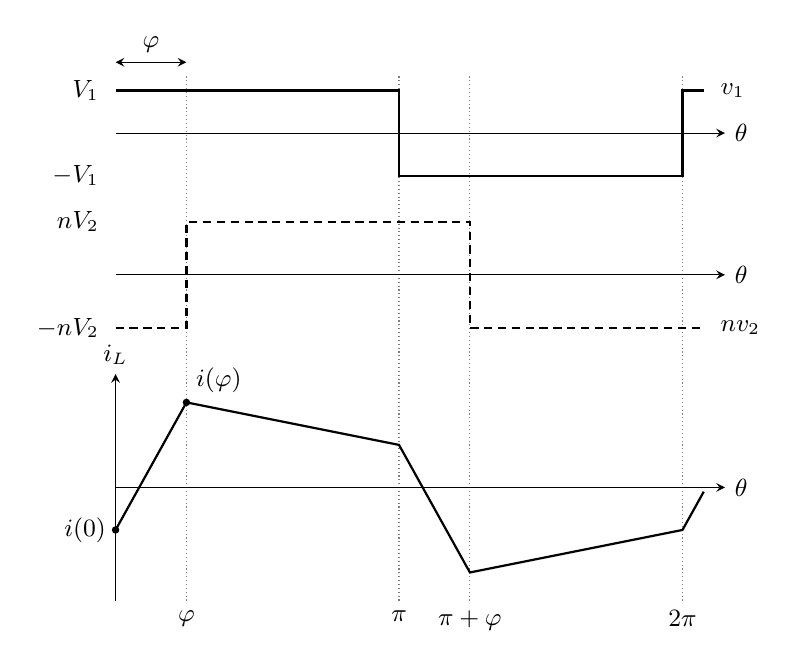
\begin{tikzpicture}[scale=0.9, >=stealth, every node/.style={font=\small}]
			% time marks
			\foreach \x/\l in {1/\varphi, 4/\pi, 5/\pi+\varphi, 8/2\pi}{
					\draw[densely dotted, gray] (\x,5.8) -- (\x,-1.6);
					\node[anchor=north] at (\x,-1.6) {$\l$};
				}
			\draw[<->] (0,6.0) -- (1,6.0) node[midway, above]{$\varphi$};
			% v1
			\draw[->] (0,5.0) -- (8.6,5.0) node[right]{$\theta$};
			\draw[thick] (0,5.6) -- (4,5.6) -- (4,4.4) -- (8,4.4) -- (8,5.6) -- (8.3,5.6);
			\node[anchor=east] at (-0.1,5.6) {$V_1$};
			\node[anchor=east] at (-0.1,4.4) {$-V_1$};
			\node[anchor=west] at (8.4,5.6) {$v_1$};
			% n v2
			\draw[->] (0,3.0) -- (8.6,3.0) node[right]{$\theta$};
			\draw[thick, densely dashed] (0,2.25) -- (1,2.25) -- (1,3.75) -- (5,3.75) -- (5,2.25) -- (8.3,2.25);
			\node[anchor=east] at (-0.1,3.75) {$nV_2$};
			\node[anchor=east] at (-0.1,2.25) {$-nV_2$};
			\node[anchor=west] at (8.4,2.25) {$nv_2$};
			% iL
			\draw[->] (0,0) -- (8.6,0) node[right]{$\theta$};
			\draw[->] (0,-1.6) -- (0,1.6) node[above]{$i_L$};
			\draw[thick] (0,-0.6) -- (1,1.2) -- (4,0.6) -- (5,-1.2) -- (8,-0.6) -- (8.3,-0.06);
			\fill (0,-0.6) circle (1.5pt) node[anchor=east]{$i(0)$};
			\fill (1,1.2) circle (1.5pt) node[anchor=south west]{$i(\varphi)$};
		\end{tikzpicture}
	\end{center}
	\caption{Bridge voltages and inductor current of the DAB with single phase shift for $d=nV_2/V_1>1$ (not to scale). The primary bridge switches at $\theta=0$, the secondary bridge at $\theta=\varphi$.}
	\label{fig:ex08_dab}
\end{figure}


\subtask{Calculate the power at $\varphi=\ang{30}$ and $V_2=\SI{12}{\volt}$, the maximum power and the currents at the switching instants.}

\begin{solutionblock}
	$P=4\cdot48\cdot12\cdot(\pi/6)(5\pi/6)/(2\pi^2\cdot\SI{1}{\mega\hertz}\cdot\SI{0.8}{\micro\henry})\,\si{\watt}=\SI{200}{\watt}$; $P_\mathrm{max}=nV_1V_2/(8f_\mathrm{sw}L)=\SI{360}{\watt}$ at $\varphi=\ang{90}$. With $V_1/(4f_\mathrm{sw}L)=\SI{15}{\ampere}$ and $d=1$: $i(0)=\SI{-5}{\ampere}$, $i(\varphi)=\SI{5}{\ampere}$.
\end{solutionblock}

\subtask{Calculate $\varphi$, $i(0)$ and $i(\varphi)$ for \SI{200}{\watt} at 10 and \SI{14}{\volt}. Check $i(\varphi)-i(0)$ with the inductor voltage during $0<\theta<\varphi$.}

\begin{solutionblock}
	$\varphi(\pi-\varphi)=2\pi^2f_\mathrm{sw}LP/(nV_1V_2)$, smaller root:
	\begin{itemize}
		\item \SI{10}{\volt} ($d=0.833$): $\varphi(\pi-\varphi)=1.645$, $\varphi=\SI{0.664}{\radian}=\ang{38.0}$; $i(0)=\SI{-7.78}{\ampere}$, $i(\varphi)=\SI{3.84}{\ampere}$ (\SI{15.4}{\ampere} in the secondary).
		\item \SI{14}{\volt} ($d=1.167$): $\varphi(\pi-\varphi)=1.175$, $\varphi=\SI{0.434}{\radian}=\ang{24.9}$; $i(0)=\SI{-2.33}{\ampere}$, $i(\varphi)=\SI{6.64}{\ampere}$.
	\end{itemize}
	During $0<\theta<\varphi$ the inductor sees $V_1+nV_2$: $\Delta i=(V_1+nV_2)\varphi/(2\pi f_\mathrm{sw}L)$, i.e.\ $\SI{88}{\volt}\cdot0.664/\SI{5.03}{\ohm}=\SI{11.62}{\ampere}$ at \SI{10}{\volt} and $\SI{104}{\volt}\cdot0.434/\SI{5.03}{\ohm}=\SI{8.98}{\ampere}$ at \SI{14}{\volt}, as from the formulas.
\end{solutionblock}

\subtask{Check the ZVS of both bridges at \SI{200}{\watt} with the current-sign criterion and with the charge criterion. Which dead time would be needed?}

\begin{solutionblock}
	Current sign: both bridges have ZVS at all three voltages. Charge: the primary needs $|i(0)|\geq2Q_\mathrm{oss}/t_\mathrm{d}=\SI{4}{\ampere}$, the secondary $n\,i(\varphi)\geq2\cdot\SI{20}{\nano\coulomb}/\SI{5}{\nano\second}=\SI{8}{\ampere}$.
	At 10 and \SI{12}{\volt} both are met. At \SI{14}{\volt} the primary has only \SI{2.33}{\ampere}: its transition takes $\SI{20}{\nano\coulomb}/\SI{2.33}{\ampere}=\SI{8.6}{\nano\second}$, and with \SI{5}{\nano\second} the primary switches turn on at partial voltage. A dead time of at least \SI{9}{\nano\second} is needed, better an adaptive one; the magnetising current of the transformer adds to $|i(0)|$ and helps the primary.
\end{solutionblock}

\subtask{Plot the ZVS boundaries over $V_2=10\ldots\SI{14}{\volt}$ for the current-sign criterion and for the charge criterion with 5 and \SI{10}{\nano\second} dead time. Calculate the rms current at \SI{200}{\watt} (notebook).}

\begin{solutionblock}
	Minimum power for full ZVS of both bridges:
	\begin{center}
		\begin{tabular}{|l|c|c|c|}
			\hline
			$V_2$                                        & \SI{10}{\volt} & \SI{12}{\volt} & \SI{14}{\volt} \\
			\hline
			current sign                                 & 92\,W          & 0              & 111\,W         \\
			charge, $t_\mathrm{d}=\SI{5}{\nano\second}$  & 153\,W         & 166\,W         & 254\,W         \\
			charge, $t_\mathrm{d}=\SI{10}{\nano\second}$ & 124\,W         & 90\,W          & 188\,W         \\
			\hline
		\end{tabular}
		\captionof{table}{ZVS boundaries of the DAB}
		\label{tab:ex08_dab}
	\end{center}
	With $d=1$ the current sign promises ZVS at every load, but with the charge criterion only the upper part of the power range is fully soft. At \SI{14}{\volt} and \SI{5}{\nano\second} even the rated power is not. The rms current at \SI{200}{\watt} is 5.56, 4.71 and \SI{4.50}{\ampere} at 10, 12 and \SI{14}{\volt}.
\end{solutionblock}

%%%%%%%%%%%%%%%%%%%%%%%%%%%%%%%%%%%%%%%%%%%%%%%%%%%%%%%%%%%%%
%% Task 4 %%
%%%%%%%%%%%%%%%%%%%%%%%%%%%%%%%%%%%%%%%%%%%%%%%%%%%%%%%%%%%%%

\task{Lagging leg of a phase-shifted full bridge}

A phase-shifted full bridge converts \SI{400}{\volt} to \SI{48}{\volt} at \SI{1}{\kilo\watt}. It has a centre-tapped rectifier and the turns ratio $n=6$. The transistors are the illustrative \SI{650}{\volt} GaN HEMTs of Lecture 2 with $C_\mathrm{oss}(v)=\SI{50}{\pico\farad}+\SI{434}{\pico\farad}\cdot e^{-v/\SI{83}{\volt}}$. Neglect the magnetising current, the transformer capacitance and the ripple of the output current.

\subtask{Calculate $Q_\mathrm{oss}$ and $E_\mathrm{oss}$ at \SI{400}{\volt}. During the transition of the lagging leg both rectifier diodes conduct and short the transformer. Which leakage inductance $L_\mathrm{lk}$ gives ZVS of the lagging leg down to 50\,\% load? Compare with an estimate based on $2E_\mathrm{oss}$.}

\begin{solutionblock}
	$Q_\mathrm{oss}=\SI{50}{\pico\farad}\cdot\SI{400}{\volt}+\SI{434}{\pico\farad}\cdot\SI{83}{\volt}\cdot(1-e^{-4.82})=\SI{55.7}{\nano\coulomb}$; $E_\mathrm{oss}=\SI{50}{\pico\farad}\cdot(\SI{400}{\volt})^2/2+\SI{434}{\pico\farad}\cdot(\SI{83}{\volt})^2\left[1-e^{-4.82}(1+4.82)\right]=\SI{6.85}{\micro\joule}$.
	With the transformer shorted, only $L_\mathrm{lk}$ drives the node. Its other end is held by the leading leg at the rail that the lagging node leaves, so $V_x=0$ in the sense of Task 8.1: $W=Q_\mathrm{oss}V_\mathrm{in}=\SI{22.3}{\micro\joule}$. At 50\,\% load the primary current is $I_\mathrm{p}=0.5\cdot(\SI{1000}{\watt}/\SI{48}{\volt})/6=\SI{1.74}{\ampere}$, so $L_\mathrm{lk}\geq2W/I_\mathrm{p}^2=\SI{14.8}{\micro\henry}$. With $2E_\mathrm{oss}=\SI{13.7}{\micro\joule}$ one would choose \SI{9.1}{\micro\henry}, 39\,\% too small.
\end{solutionblock}

\subtask{Calculate the duty-cycle loss at full load for 200\,kHz and \SI{1}{\mega\hertz}. Can the converter deliver \SI{48}{\volt} at \SI{1}{\mega\hertz}?}

\begin{solutionblock}
	At the start of each power interval the primary current reverses from $+I_\mathrm{p}$ to $-I_\mathrm{p}$ ($I_\mathrm{p}=\SI{3.47}{\ampere}$ at full load) with the slope $V_\mathrm{in}/L_\mathrm{lk}$; meanwhile both diodes conduct and no power is transferred: $\Delta t=2I_\mathrm{p}L_\mathrm{lk}/V_\mathrm{in}=\SI{257}{\nano\second}$.
	Relative to the half period: $\Delta D=4L_\mathrm{lk}I_\mathrm{p}f_\mathrm{sw}/V_\mathrm{in}=0.10$ at \SI{200}{\kilo\hertz} and 0.51 at \SI{1}{\mega\hertz}. The required duty cycle $D=nV_\mathrm{o}/V_\mathrm{in}+\Delta D$ is 0.82 at \SI{200}{\kilo\hertz}, but 1.23 at \SI{1}{\mega\hertz}: impossible. A wide ZVS range and MHz operation exclude each other in the PSFB; Lecture 9 shows converters that avoid the conflict.
\end{solutionblock}

\subtask{Why does the leading leg keep ZVS down to light load?}

\begin{solutionblock}
	During the transition of the leading leg the transformer still transfers power. The reflected output current $I_\mathrm{o}/n$ drives the node as a stiff current, with the energy of the output inductor behind it. Only the lagging leg depends on the energy of $L_\mathrm{lk}$.
\end{solutionblock}

%%%%%%%%%%%%%%%%%%%%%%%%%%%%%%%%%%%%%%%%%%%%%%%%%%%%%%%%%%%%%
%% Task 5 %%
%%%%%%%%%%%%%%%%%%%%%%%%%%%%%%%%%%%%%%%%%%%%%%%%%%%%%%%%%%%%%

\task{ZVS of your brief (homework)}

Prepare the soft-switching part of milestone M2 (16.12.).

\subtask{List every switching instant of your converter, the current that drives each transition and the inductance whose energy it uses. Check direction, charge and energy at the worst-case operating point.}

\begin{solutionblock}
	Check list: current direction towards the switch that turns on next; $2Q_\mathrm{oss}$ plus transformer, winding and layout capacitance within $t_\mathrm{d}$; $\frac{1}{2}LI^2\geq Q_\mathrm{oss}(V-2V_x)$ when the current is not stiff. The worst case is usually light load, and for a DAB or LLC the extreme of the voltage range.
\end{solutionblock}

\subtask{Choose the dead times (fixed or adaptive) and estimate the remaining switching loss: partial ZVS, reverse conduction, $C_\mathrm{oss}$ hysteresis and turn-off overlap.}

\begin{solutionblock}
	A fixed dead time must cover the slowest transition and costs reverse conduction ($V_\mathrm{SD}\cdot I\cdot\Delta t\cdot f_\mathrm{sw}$ per transition) at the fast ones; adaptive dead time (Lecture 4) avoids this. The $C_\mathrm{oss}$ hysteresis loss is taken from measured data (Lectures 2 and 5).
\end{solutionblock}

\vspace{0.5cm}
Remark: The notebook \texttt{tutorialEx08\_task.ipynb} simulates the ZVS transition (Task 8.1), the TCM converter with its dead time (Task 8.2) and the ZVS boundaries of the DAB (Task 8.3), and shows the leakage-inductance trade-off of the PSFB (Task 8.4).
